\documentclass{article}
\usepackage{graphicx} % Required for inserting images
\usepackage[utf8]{inputenc}
\usepackage[spanish]{babel}
\usepackage{xcolor}
\usepackage{amsmath}
\usepackage{titling}

\setlength{\parindent}{0pt}
\pagecolor{black}
\color{white}
\title{
    % 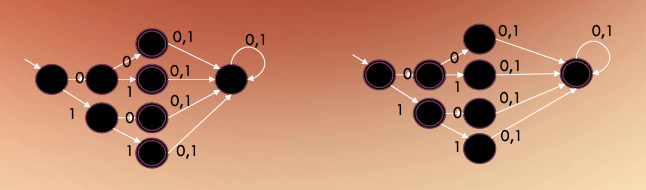
\includegraphics[width=10cm]{../imgs/AFD complemento.png}
    \textbf{Teoría de la computación}
}
\author{BlasAST}
\date{May 2025}

\begin{document}
\maketitle

\newpage

\tableofcontents

\newpage

\section{Maquina de Turing Universal}

La idea base de esto es que podemos poner (codificar) una MT en la
cinta de otra mostrando las transiciones de la MT
realizadas mediante su alfabeto y su input.

De esta forma forma se crea la $MTU$ y esta se pondrá a leer y
ejecutará las intrucciones que encuentre en la cinta, las cuales
describen el funcionamiento de la MT. A partir del input, también
presente en la cinta la $MTU$ simulará el comportamiento de la MT
escribiendo los resultados parciales y finales en otra porción de
la cinta.

\begin{quote}
    Otra forma de verlo es que una MTU es basicamente un emulador
    que simula $X$ consola.
\end{quote}

Este formalismo de MTU nos permite hacer maquinas que ejecuten otras
maquinas. Se utiliza diariamente para:
\begin{itemize}
    \item En el Hardware (Cargamos aplicaciones sobre nuesto S.O,
    incluso el propio S.O es una MT)
    \item Intérpretes. Capaces de aceptar programas escritos
    en un lenguaje de programación de alto nivel como Python.
    \item Emuladores y Maquinas virtuales.
\end{itemize}

\newpage

\section{Concepto de Algoritmo}

Un algoritmo puede tener varios tipos de definiciones pero siempre
tiene el mismo significado:

\begin{itemize}
    \item \textbf{La forma más facil de entenderlo es la siguiente.}
    Informalmente es una secuencia de pasos finitos que resuelven un
    problema.
    \item Más formalemnte es una secuencia finita de pasos que
    calculan una determinada función.
    \item La definición más formal sería: Toda aquella computación
    capaz de ser realizada en una MT
\end{itemize}

\section{Computabilidad y Decibilidad}

Una vez entendemos que es un algoritmo podemos pasar a entender que
es \textbf{su computabilidad y decibilidad.}\\

Un algoritmo es computable cuando para cualquier input podemos obtener
su output. Es decir, es un algoritmo \lq resolvible\rq \space que resuelve dado que
mediante el input que reciba y una cantidad finita de pasos termina y
devuelve el resultado del computo.\\\\

Un algoritmo es decidible si con el input que recibe es capaz de
determinar si dicho input pertenece o no al lenguaje. Devuelve
respuestas binarias (accept, reject). \textbf{Si un algorimto es
decidible es siempre computable.}\\

Para saber si es decidible la MT que reconoce dicho lenguaje del
algoritmo debe ser capaz de terminar el programa aceptando todos los
inputs, en caso contrario se rechaza la palabra.\\\\

Por último un algoritmo es semidecidible cuando hay una MT que decide.

Termina siempre que se acepta la palabra del input y si no la acepta,
es decir, el input no pertenece al lenguaje, puede rechazar la palabra
o no terminar nunca.

\newpage

\section{Problema de la parada (HALTING PROBLEM)}

Supongamos que tenemos una MTU que nos puede devolver 2 cosas. Si la MTU termina
nos devuelve True mientras que si la MTU no termina nos devuelve False. Pues bien,
esta MTU tiene un  problema a pesar de estar bien definida siguiendo las reglas
de la definición de MT.\\

\[
\text{Una MTU sería asi}
\left\{
    \begin{array}{l}
        $true$ \text{ si MT(x) termina}\\
        $false$ \text{ si MT(x)} \uparrow \text{ (no termina)}
    \end{array}
\right.
\]

Pero, si tratamos de construir una MTU que sea capaz de decirnos \textbf{siempre}
si \textbf{cualquier} MT termina o no. Podemos darnos cuenta de que no es posible
crear este tipo de MT.


Para explicarlo mejor se puede encontrar un contraejemplo de dicha MTU. Suponemos
que esta MTU existe, lo que quiere decir por contraejemplo que lo contrario es
verdadero y por ello también supondremos que no existe una MTU que cumpla esta
condición.\\

En lógica se expresaría de la siguiente forma:\\\\
$ Termina(MTU)\leftrightarrow \neg Termina(MTU)$

\begin{quote}
    Imaginemos que tenemos una MTU que termina cuando MT no termina
    y no termina cuando MT termina.
\end{quote}
Ojo, true o false es el valor final,
internamente termina cuando no termina y no termina cuando termina.
\[
\text{MTU(MT,x).}
\left\{
    \begin{array}{l}
        false \text{ si MT(x)} \uparrow \text{(no termina)}\\
        true \text{ si MT(x) termina}
    \end{array}
\right.
\]

Pues si ahora le pasamos a ella misma como MT tendriamos lo siguiente

\[
\text{MTU(MTU,x)}
\left\{
    \begin{array}{l}
        false \text{ si MTU(X)} \uparrow \text{(no termina)} \\
        true \text{ si MTU(X) termina}
    \end{array}
\right.
\]

El resultado de esto sería una contradicción dado que al aplicarse lo contrario del
resultado internamente terminaria cuando no termina o terminaria cuando no termina
lo cual entraría en un bucle.\\\\

Debido a esto la conclusión es que no existe una MT capaz de decirno si cualquier MT
(incluso ella misma) termina o no.\\

Lo que si podemos hacer son demostraciones a mano o con una MT para demostrar que otra
MT concreta termina o no. Esto es parte del estudio del área de Verificación de Software.

\section{Reducibilidad}
Para resolver un problema a veces puede ser útil simplificarlo en otros problemas
más pequeños que sepamos resolver.\\

Esta idea se basa en tratar de demostrar que el problema que queremos resolver
es en realidad otro caso en particular de otro problema que ya sabemos como
resolverlo. $P_n \subseteq P_c$\\

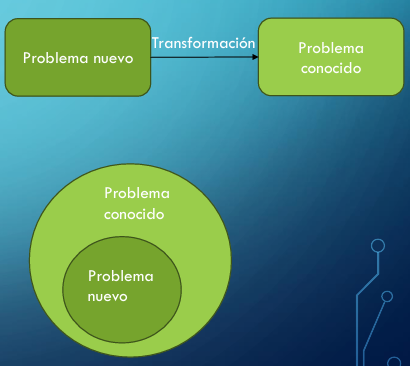
\includegraphics[width=200px]{../imgs/reducibilidad.png}

Generalmente es necesario realizar transformaciones al nuevo problema para
expresarlo en términos del problema conocido. Una forma de hacerlo es mediante
la inclusión de lenguajes.

\section{Inclusión de lenguajes}
Una vez tenemos dos lenguajes podemos ver si un lenguaje esta contenido en otro.
Esto se resuelve normalmente haciendo el complemento del lenguaje más general y
haciendo la intersección de ambos y posteriormente si la intersección de ambas
es vacía.\\

Lo anterior como formula sería:\\

$\mathcal{L}(P_n) \subseteq \mathcal{L}(P_c) \leftrightarrow 
\overline{\mathcal{L}(P_c)} \cap \mathcal{L}(P_n) = \emptyset$

\newpage

\section{Otros formalismos}

Existen otros formalismos de computación equivalentes en poder expresivo
al igual que las MT. Algunas son:\\

\begin{itemize}
    \item Cálculo Lambda
    \item Lenguajes Formales
    \item Funciones Parcialmente Recursivas
    \item Variaciones de MT: Varias cintas, cintas bidimensionales, etc.
    \item Autómatas finitos con dos pilas o con dos contadores
    \item Maquina de post
    \item Autómatas celulares
    \item El juego de la Vida de John Conway
    \item Computador cuántico
    \item Lenguajes de programación modernos si tuvieran memoria ilimitada.
\end{itemize}

\section{Tesis de Church-Turing}

La tesis de Church Turing establece que una MT es capaz de computar/ejecutar
todo aquiello a lo que se le puede llamar algoritmo. Pasa lo mismo con el
Cálculo Lambda creado por Church, siendo igual de expresivas que las MTs y por
ello se hace la tesis de que ambas abarcan todo lo que es efectivamente un
algoritmo en su definición más amplia.\\

Dado a que todavía no ha sido demostrado sigue siendo una tesis porque el
concepto de algoritmo no pertenece a ninguna clase mátematica y no se puede
realizar la demostración.

Casi todos los matemáticos e informáticos lo dan por verdadero y consideran
que es la frontera entre lo computable(algoritmo) y lo no computable (todo
aquello que ni una MT puede calcular)\\

Todos los formalismos equivalentes a una MT cumplen:

\begin{itemize}
    \item Realizan una cantidad finita de trabajo en cada paso.
    \item Acceso aleatorio (a no ser que se usen X operaciones) a memoria
    finita.
\end{itemize}
\end{document}